\documentclass[a4paper, oneside, onecolumn, 11pt]{memoir}
\newenvironment{code}{\captionsetup{type=listing}}{}

%\begin{code}
%    \caption{Den skrevne Pythonkode.
%    \label{kode}}

%    \inputminted[firstline=20, lastline=30,
%        frame=single, framesep=2mm, fontsize=\footnotesize, linenos% Spanning over more than one page!
%    ]{python}{kode.py}
%\end{code}

% Preamble
\usepackage{preamble}

%\graphicspath{~/graphics/}

\title{Logbook}
\author{Anne Kirstine Knudsen\thanks{email} \and Laurits N. Stokholm\thanks{laurits.stokholm@post.au.dk}}
\date{\today}

\begin{document}
\maketitle
%\tableofcontents
\section{Problem}
% What is the problem


\subsection{Research method \#1}
Optical detector\ldots
\subsubsection{Planning}
% Start each entry by stating what you are planning to do


Beamsize: We used a slit of variable width. $1, 2, 3, 4, 5$

\subsubsection{Experimental Equipment Available}
% What is the experimental 
\begin{itemize}
    \item Ruler
    \item %Red diode Laser $650 \si{\nano\meter}$
    \item Collimating slits with 5 slits
    \item Polarizer with rotational mount
    \item Polarizer
    \item Collimating lens
    \item Rotational mount
    \item High sensitivity light sensor
    \item PicoScope
\end{itemize}

\subsubsection{Critical issues}
% What are the critical issues?
Intensity of light is half s- and p-polarized.
Allignment of detector and laserbeam.

\subsubsection{Strategy}
% How to carry out the tasks
% Strategy for carry out the experiments
% - which parameter have to be meassured and how to best do it
% - taking reflections into account

\subsection{Setup}
% Make a sketch of the experiment, explain why this setup.

\subsection{Laboratory setyp}
% Does it work as expected
% Did you chose to go differently than originally sketched?
% Add pictures
\begin{figure}[h]
    %\label{fig:setup}
    \centering
    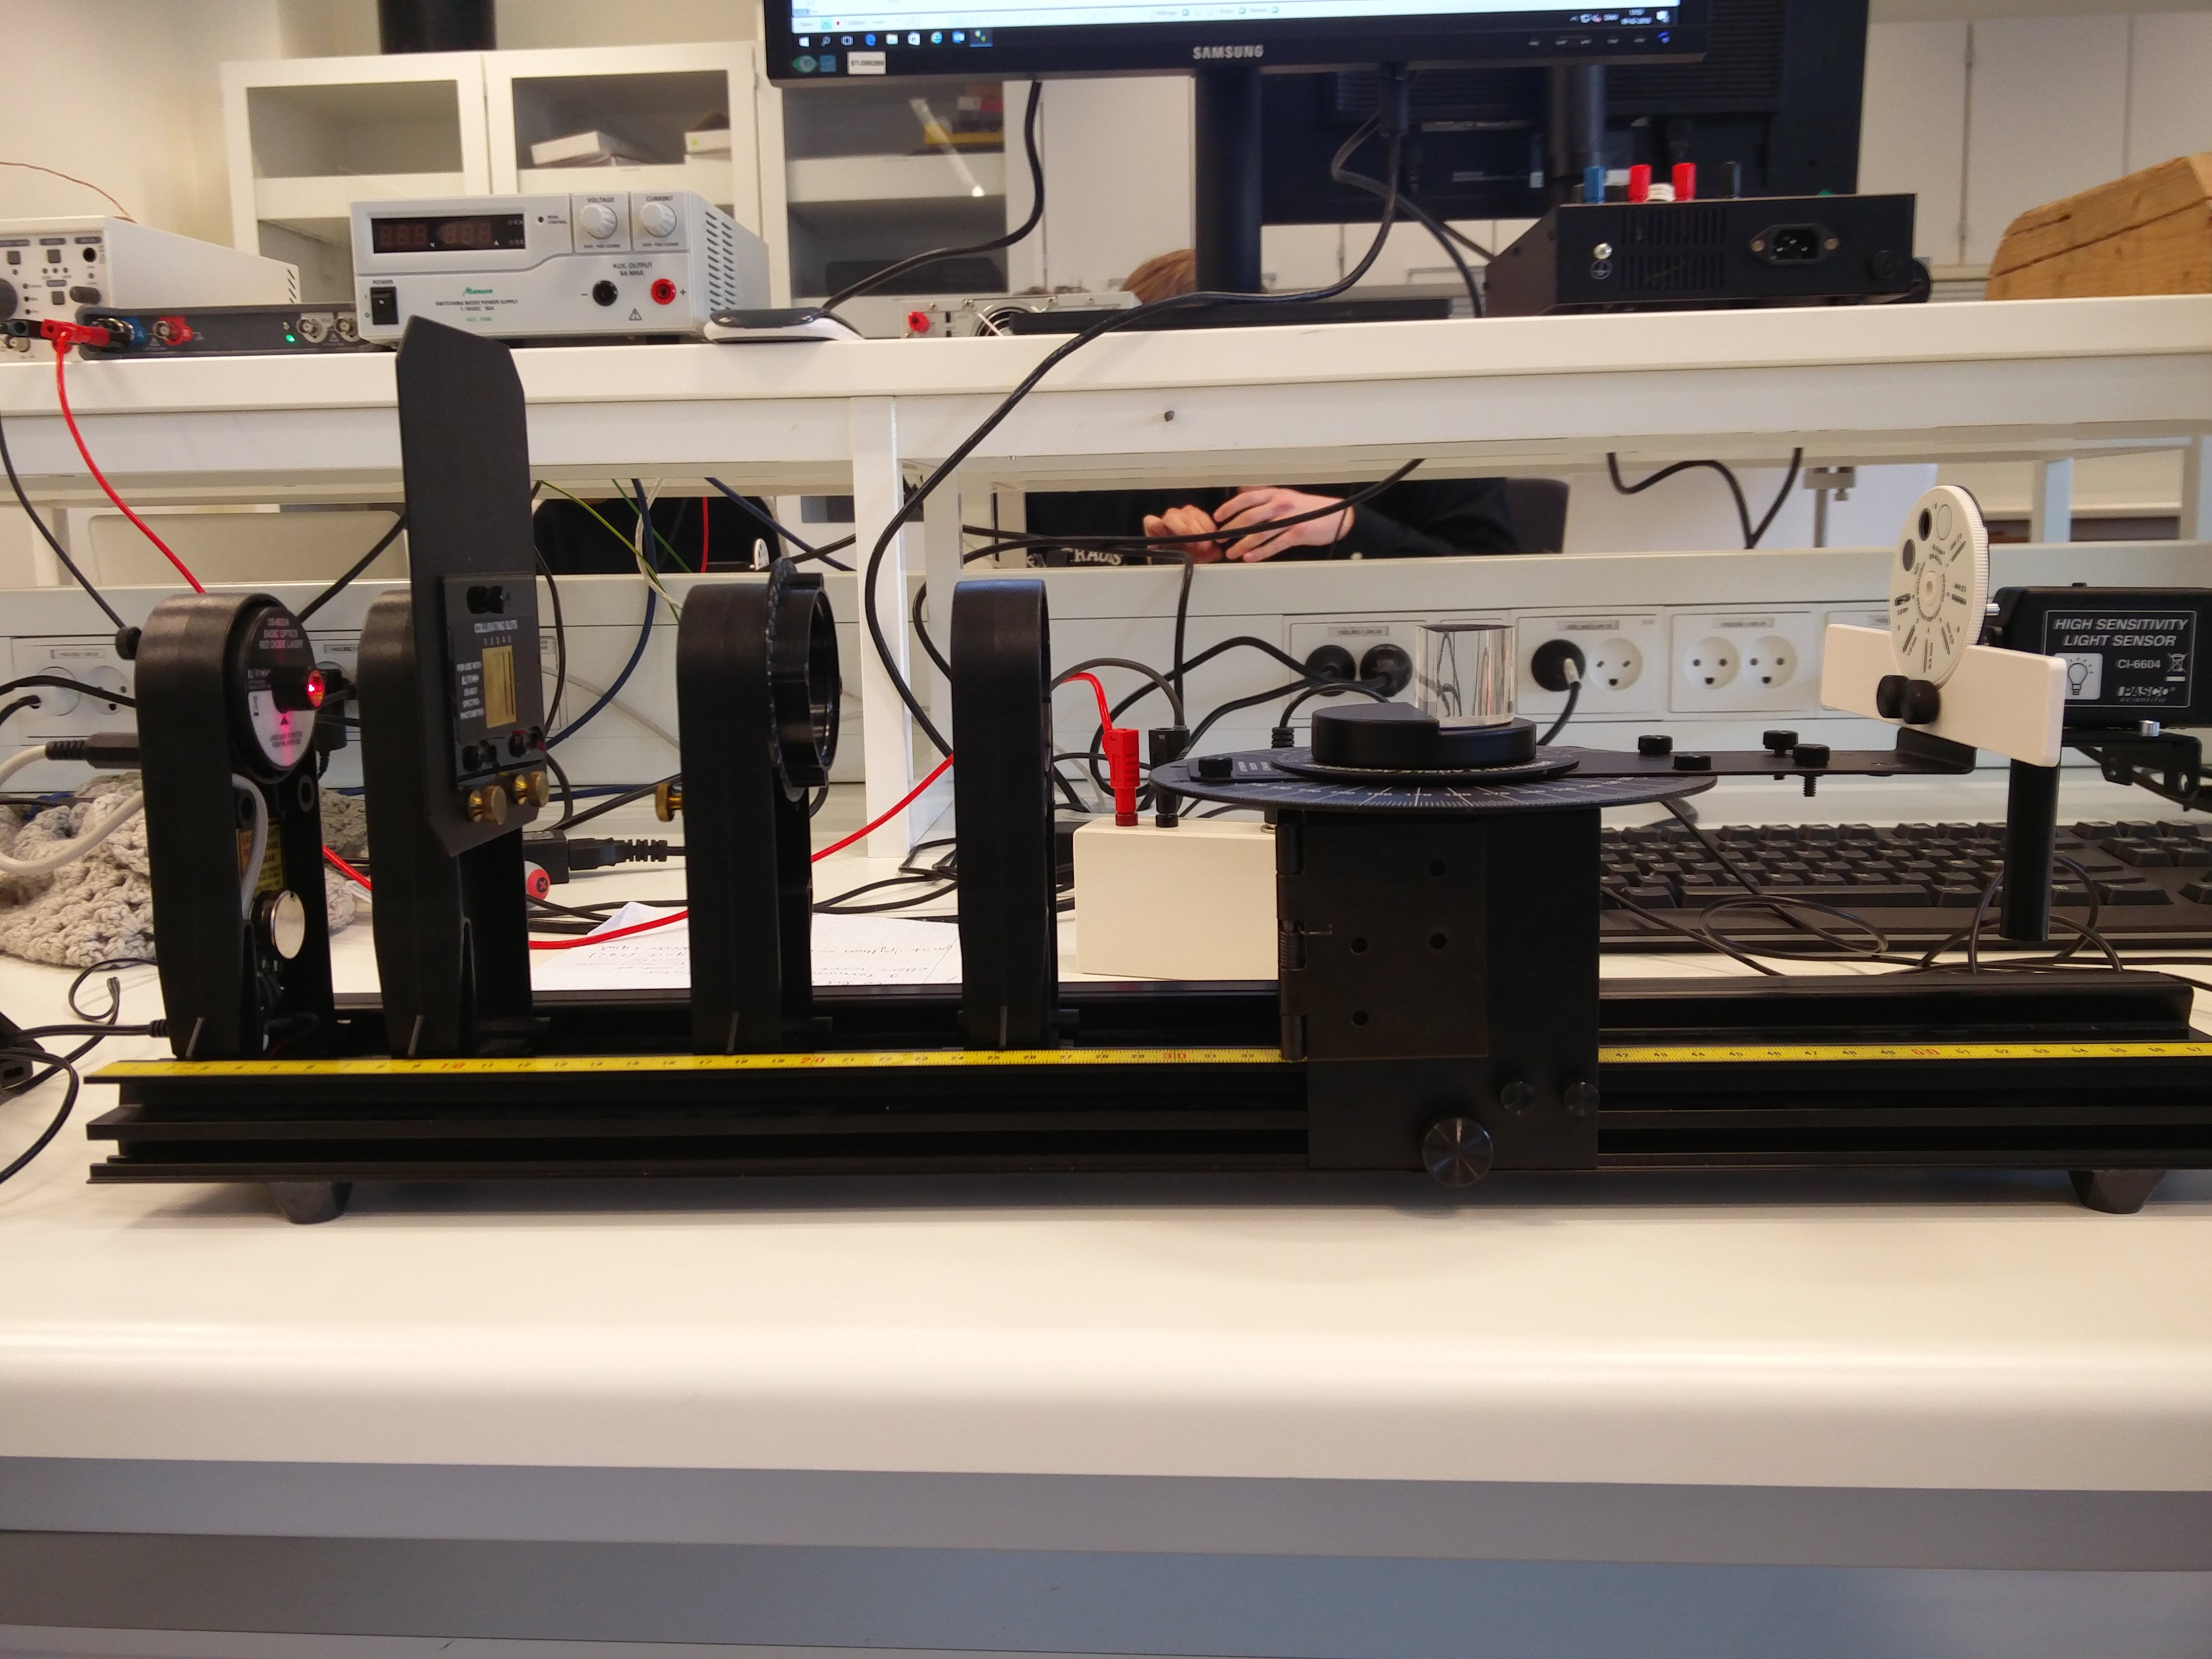
\includegraphics[width=\textwidth]{setup}
    \caption{Look at me I am a caption!}
\end{figure}

\subsection{Raw data}
% Screen shots and link to data files

% 1st Meassurement
%slit width 2, 0.5 mm

\subsection{Fast analysis}
% Does the data seem to be valid?
% Do you see any sign of systematic errors?

\subsection{Conclusion}
% What have you learned?
% What has or could be done differently for improving the results?
Her og der og alle vegne, som du kan se på \cref{SourceCode:1}

\begin{code}
	\caption{Caption
    \label{SourceCode:1}}
    \inputminted[firstline=1, lastline=5, frame=single, framesep=2mm, fontsize=\footnotesize, linenos% Spanning over more than one page!
]{python}{kode.py}
\end{code}

\end{document}

